\documentclass[Journal,letterpaper,InsideFigs,NoLists,NoLineNumbers]{ascelike-new}
\WarningFilter{caption}{Unknown document class}
\usepackage[utf8]{inputenc}
\usepackage[T1]{fontenc}
\usepackage{lmodern}
\usepackage{graphicx}
\usepackage[style=base,figurename=Fig.,labelfont=bf,labelsep=period]{caption}
\usepackage{amsmath}
\usepackage{newtxtext,newtxmath}
\usepackage[colorlinks=true,citecolor=red,linkcolor=black]{hyperref}
\usepackage{bm,textcomp,url}
\urlstyle{same}
\graphicspath{{figs/}}
\NameTag{Anticona, \today}
\renewcommand{\thefigure}{S\arabic{figure}}
\renewcommand{\thetable}{S\arabic{table}}
\begin{document}
\title{Supplemental Materials\\[0.5ex] Leps-P: Probabilistic Strength Envelopes with Stress-Decaying Curvature for Rockfill and Mine Waste Rock}
\author[1]{Wilson A. Anticona}
\affil[1]{\textbf{[ASCE grade, affiliation, and e-mail to be completed]}}
\maketitle
\noindent This file contains Figs.~S1--S5 and Tables~S1--S2, cited in the paper. Equation and table numbers without the prefix S refer to the paper.

\begin{figure}[htbp]
\centering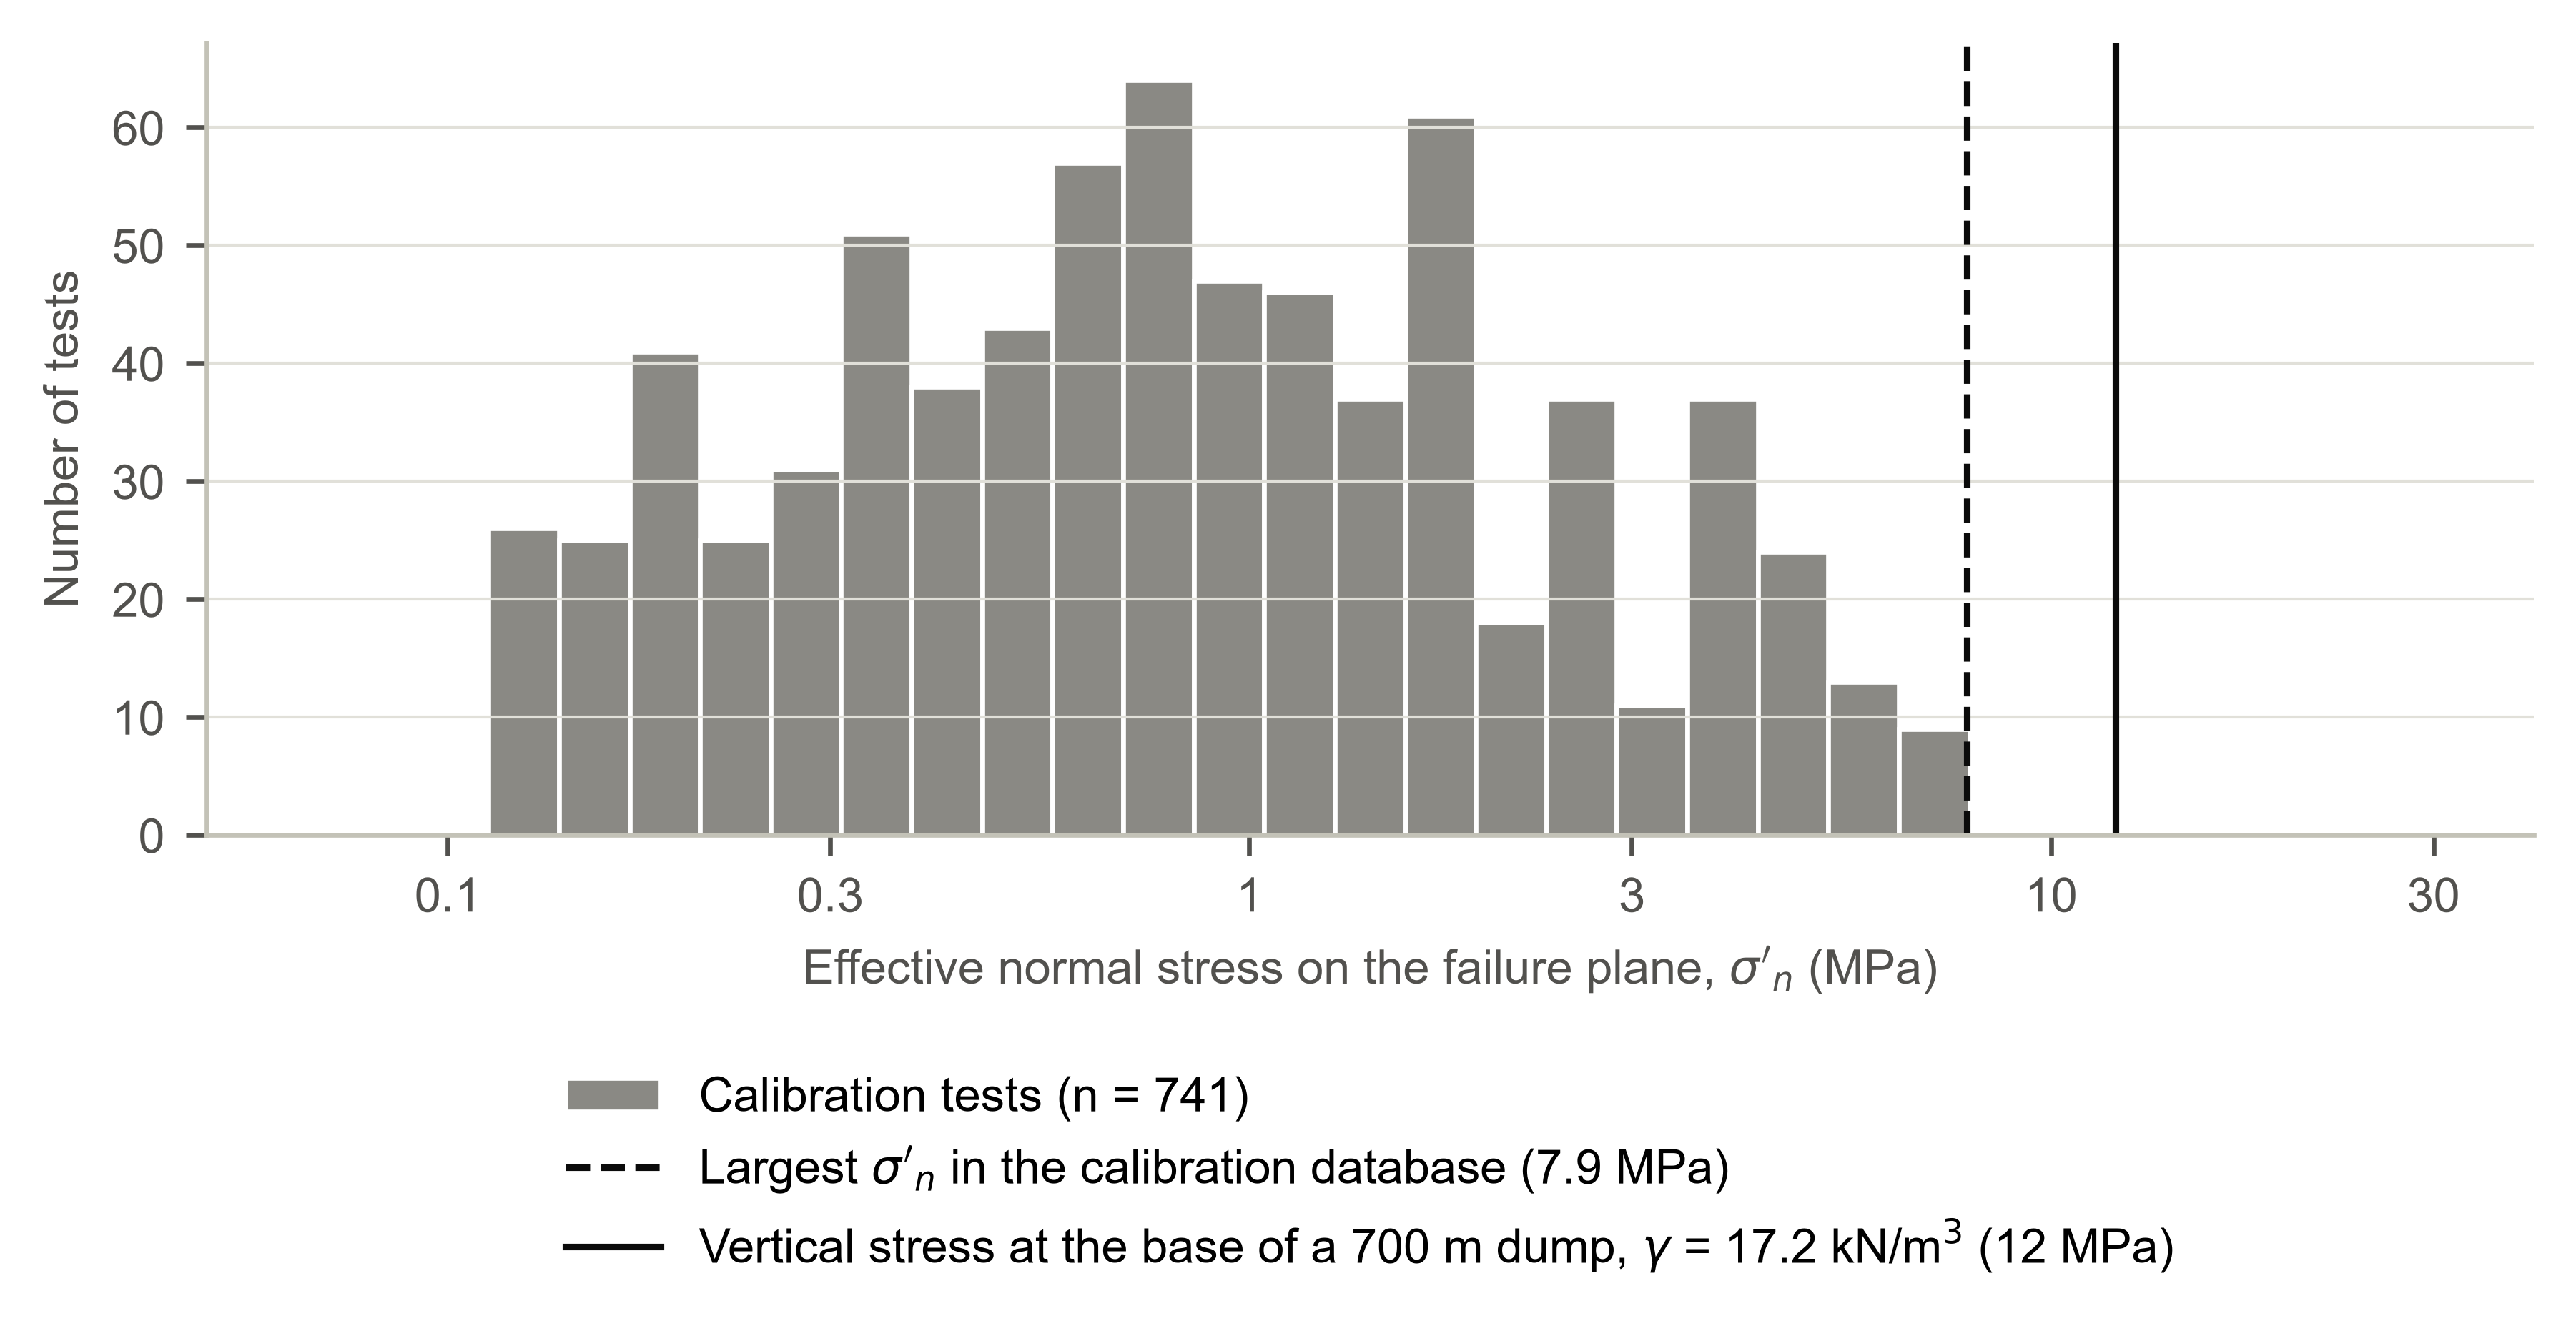
\includegraphics[width=6.0in]{FigS1_stress_coverage.png}
\caption{Distribution of effective normal stress on the failure plane in the calibration database.}
\end{figure}
\clearpage
\begin{figure}[htbp]
\centering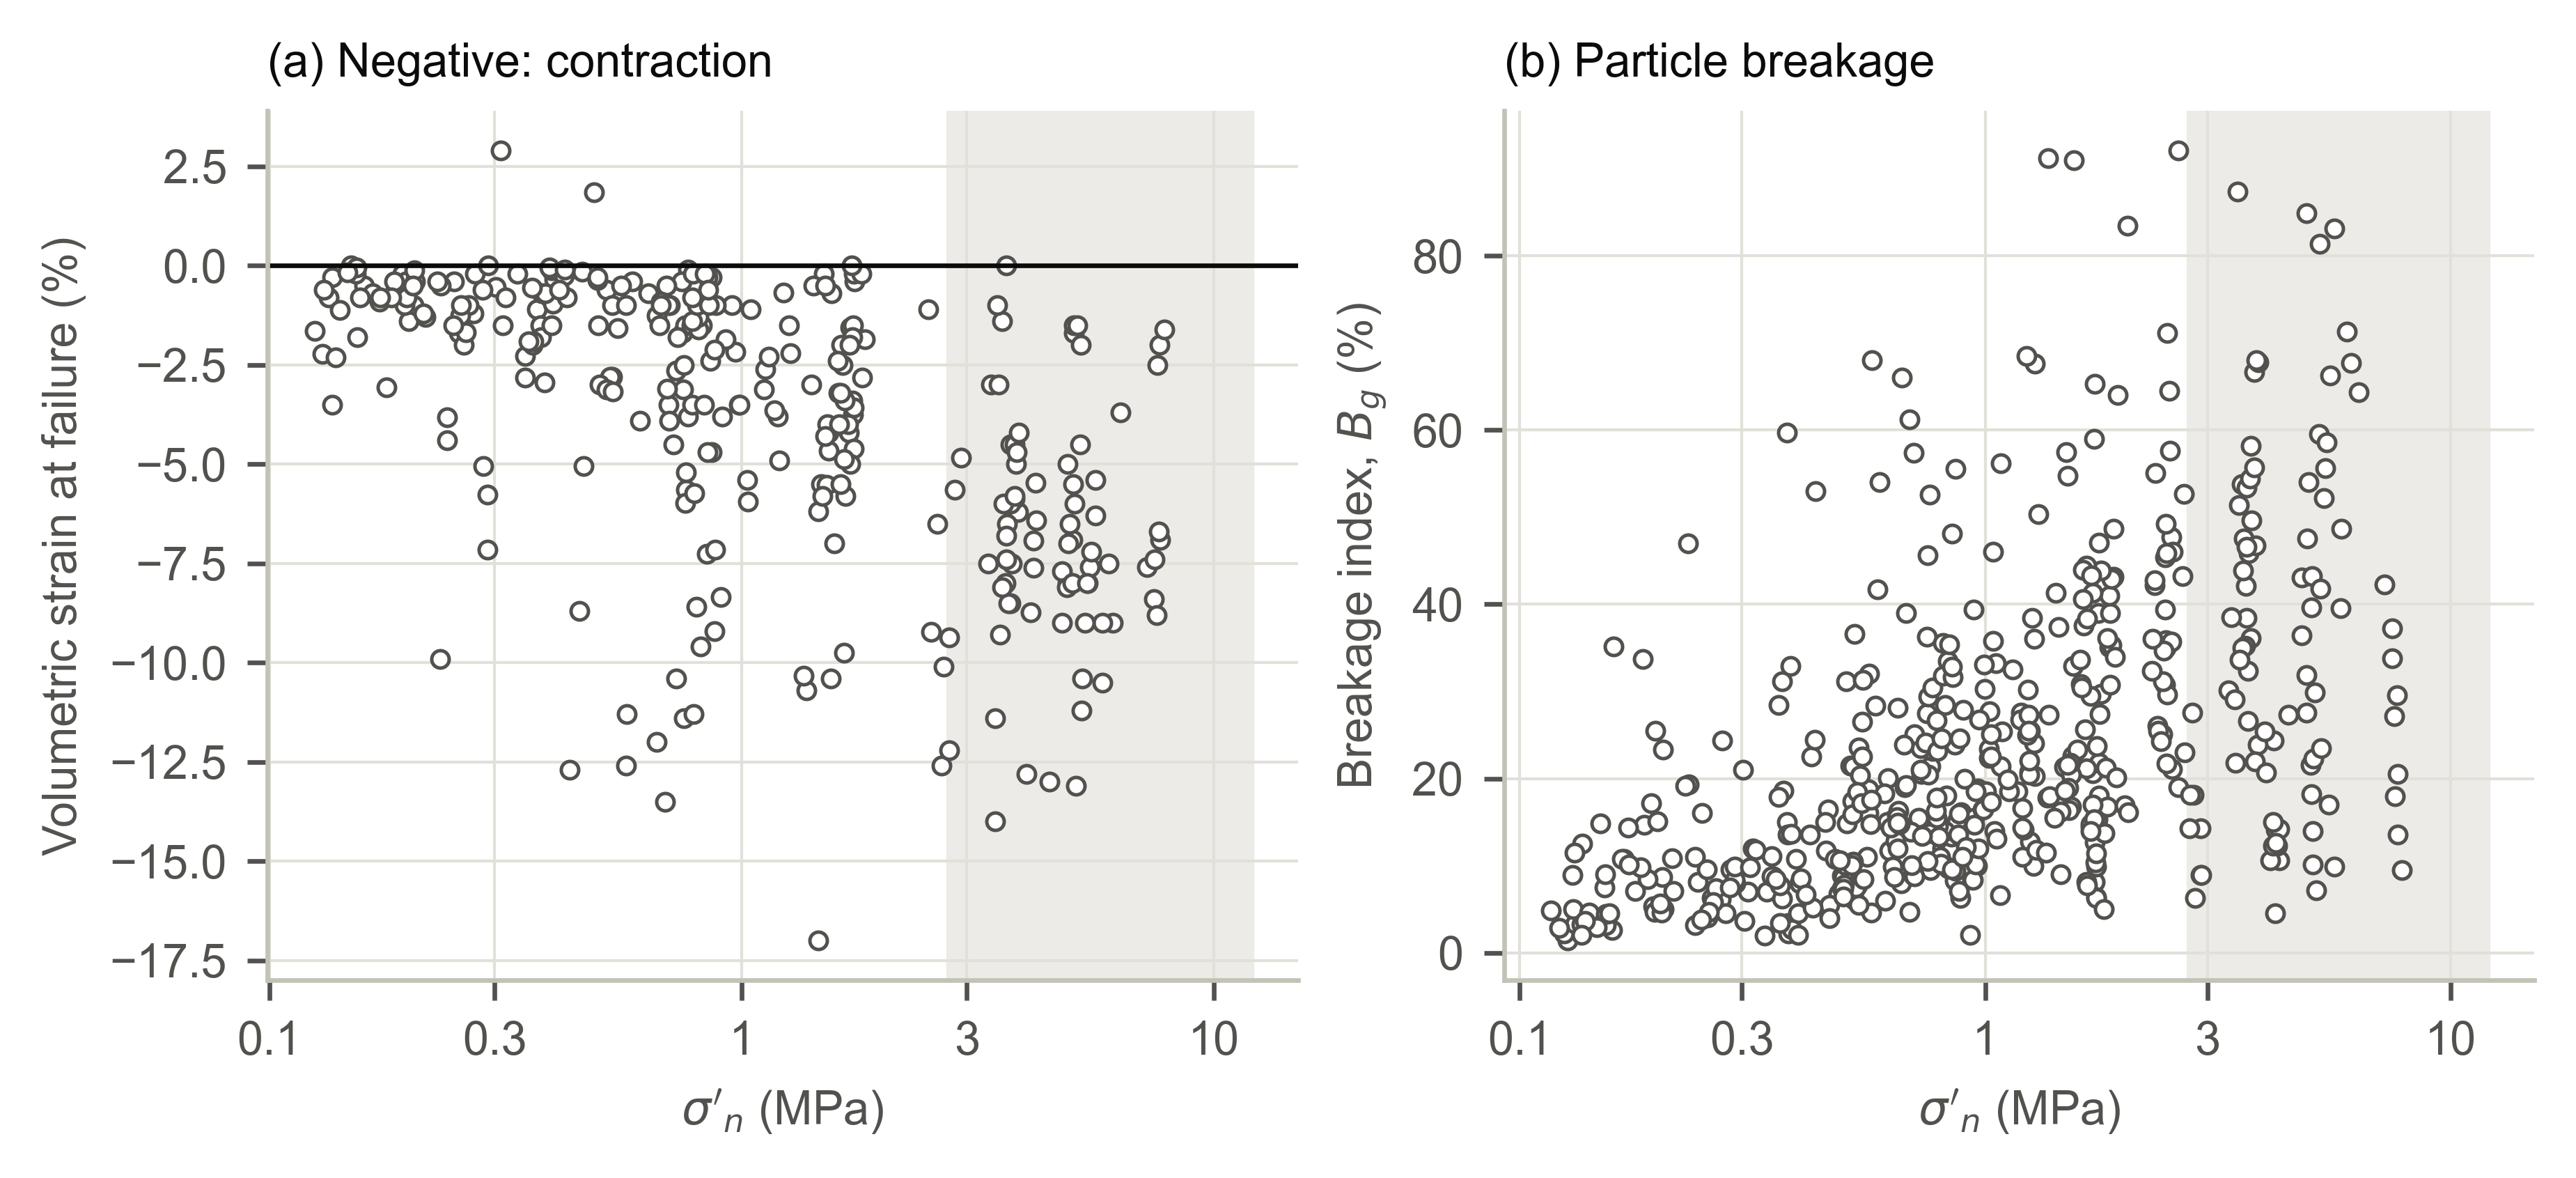
\includegraphics[width=6.0in]{FigS2_volumetric_breakage.png}
\caption{Net volumetric strain at the maximum deviator (negative: contraction) and breakage index of Marsal (1973) versus $\sigma'_n$ in the calibration database; shaded: $\sigma'_n$ > 2.75 MPa. Reported breakage indices above 100\%, which are impossible by definition, were excluded (4 tests). Above 2.75 MPa the residuals of Leps-P were unrelated to the breakage index (Spearman $\rho$ = 0.00, n = 91).}
\end{figure}
\clearpage
\begin{figure}[htbp]
\centering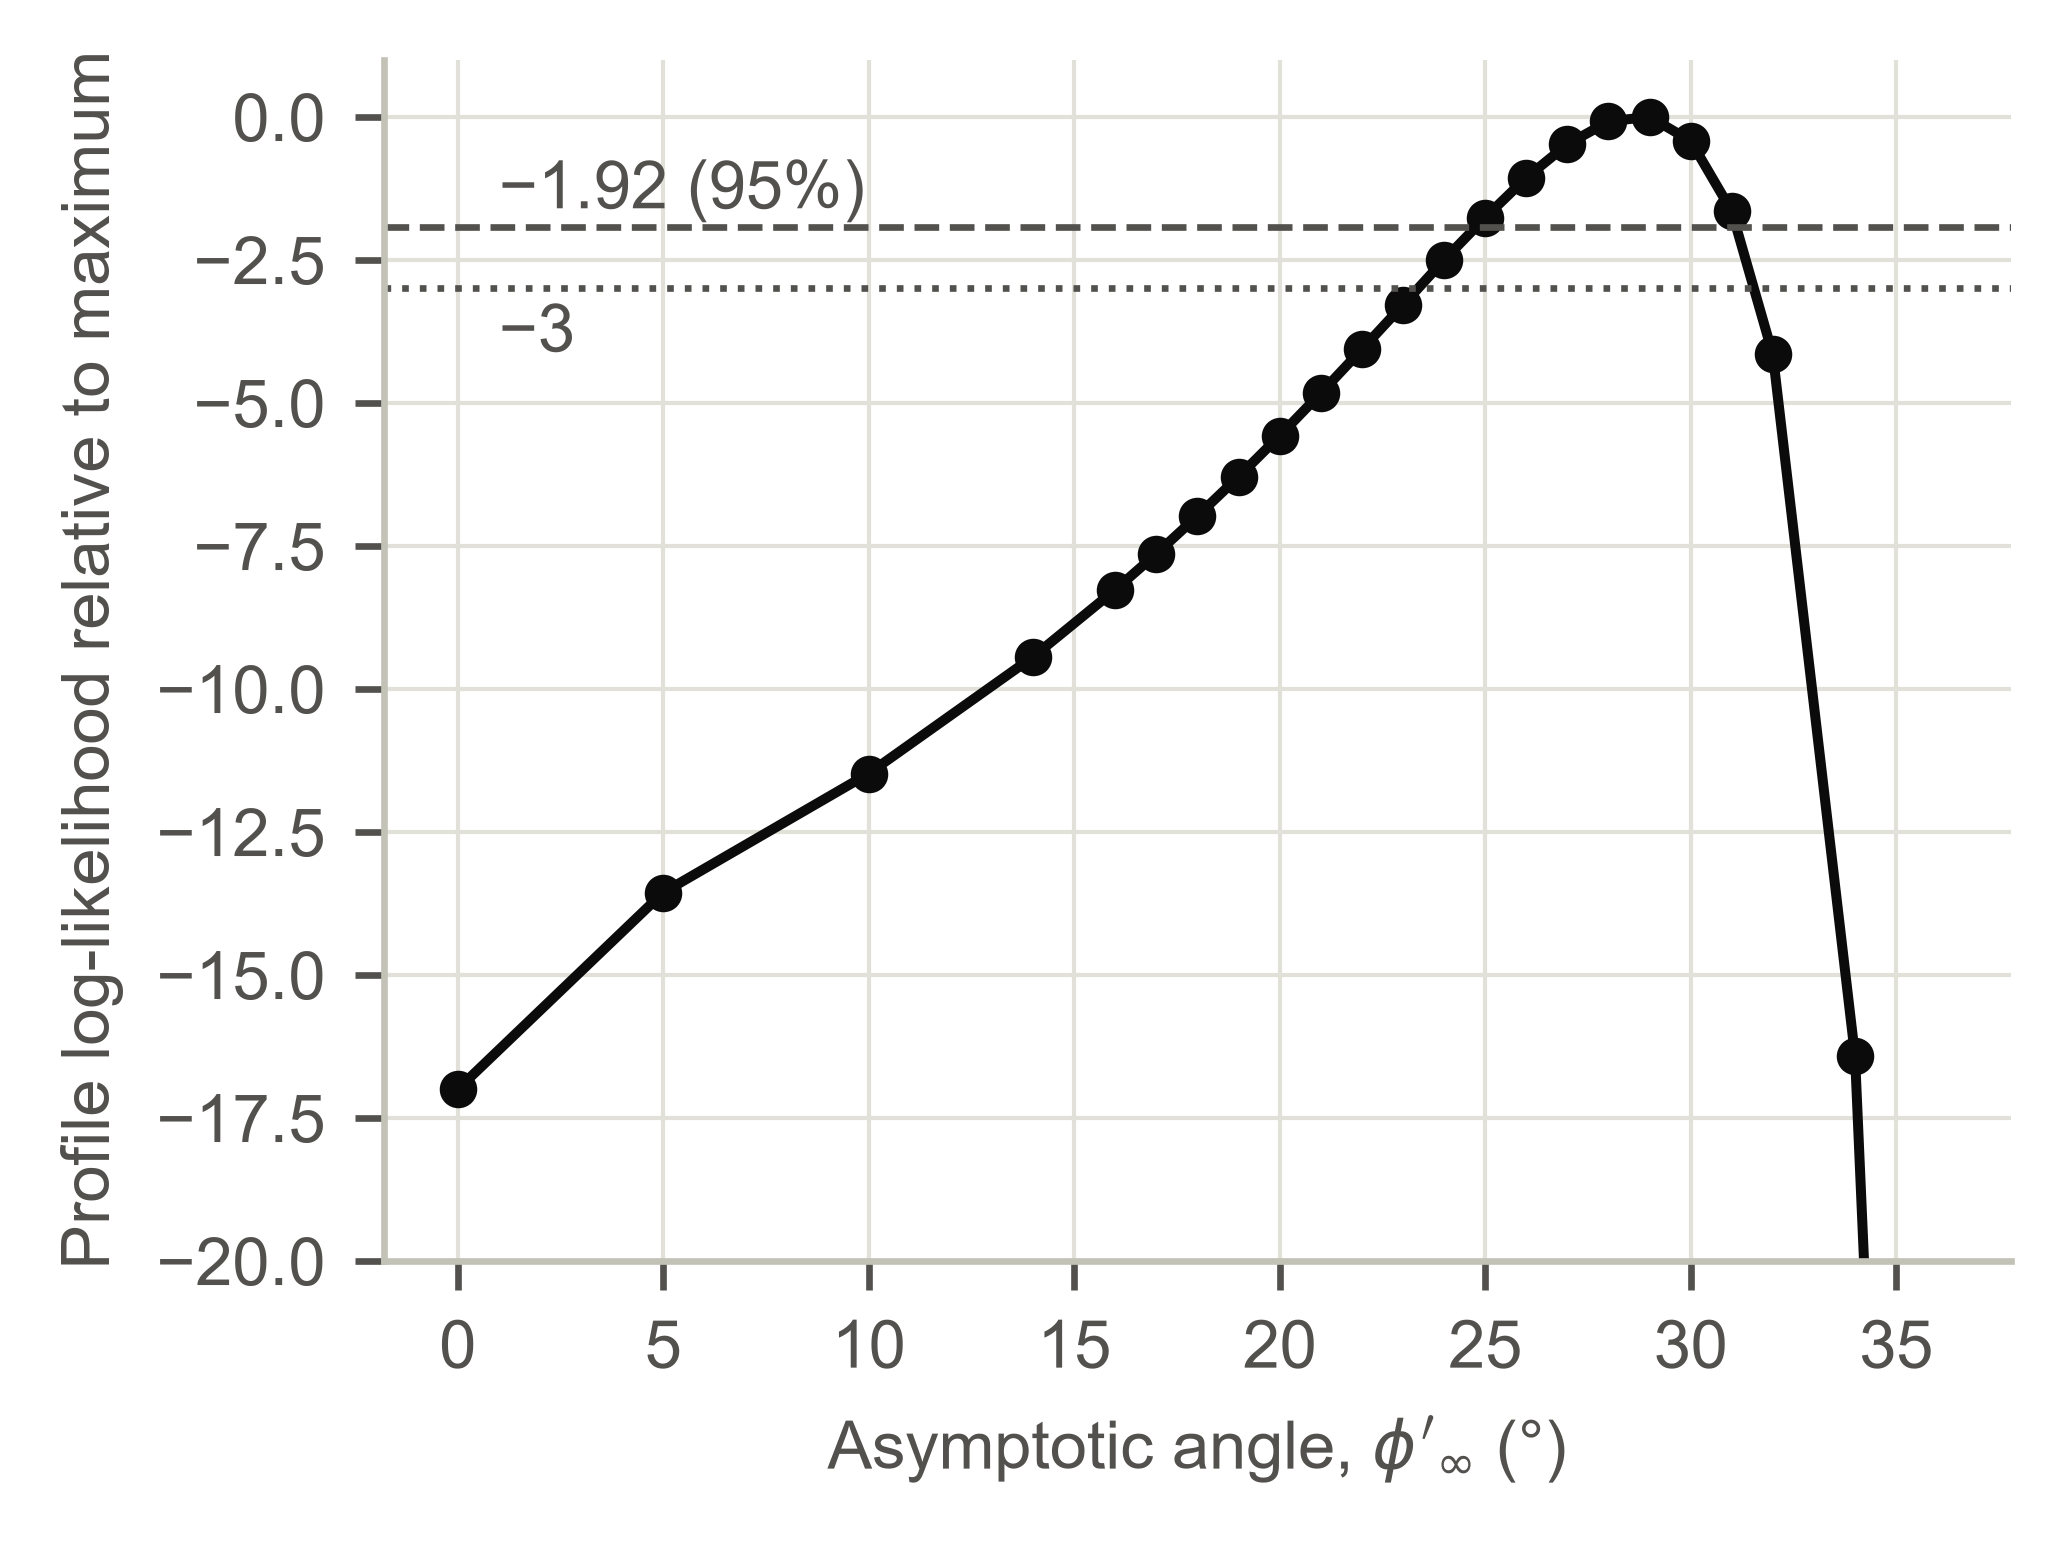
\includegraphics[width=4.0in]{FigS3_profile_likelihood.png}
\caption{Profile log-likelihood of the asymptotic angle $\phi'_\infty$ relative to its maximum (1685.51); at each angle the population decay rate $\zeta_0$ and the variance parameters were re-estimated by maximum likelihood. $\phi'_\infty$ = 0 corresponds to the form without an asymptote. Dashed: 3 log-likelihood units below the maximum.}
\end{figure}
\clearpage
\begin{figure}[htbp]
\centering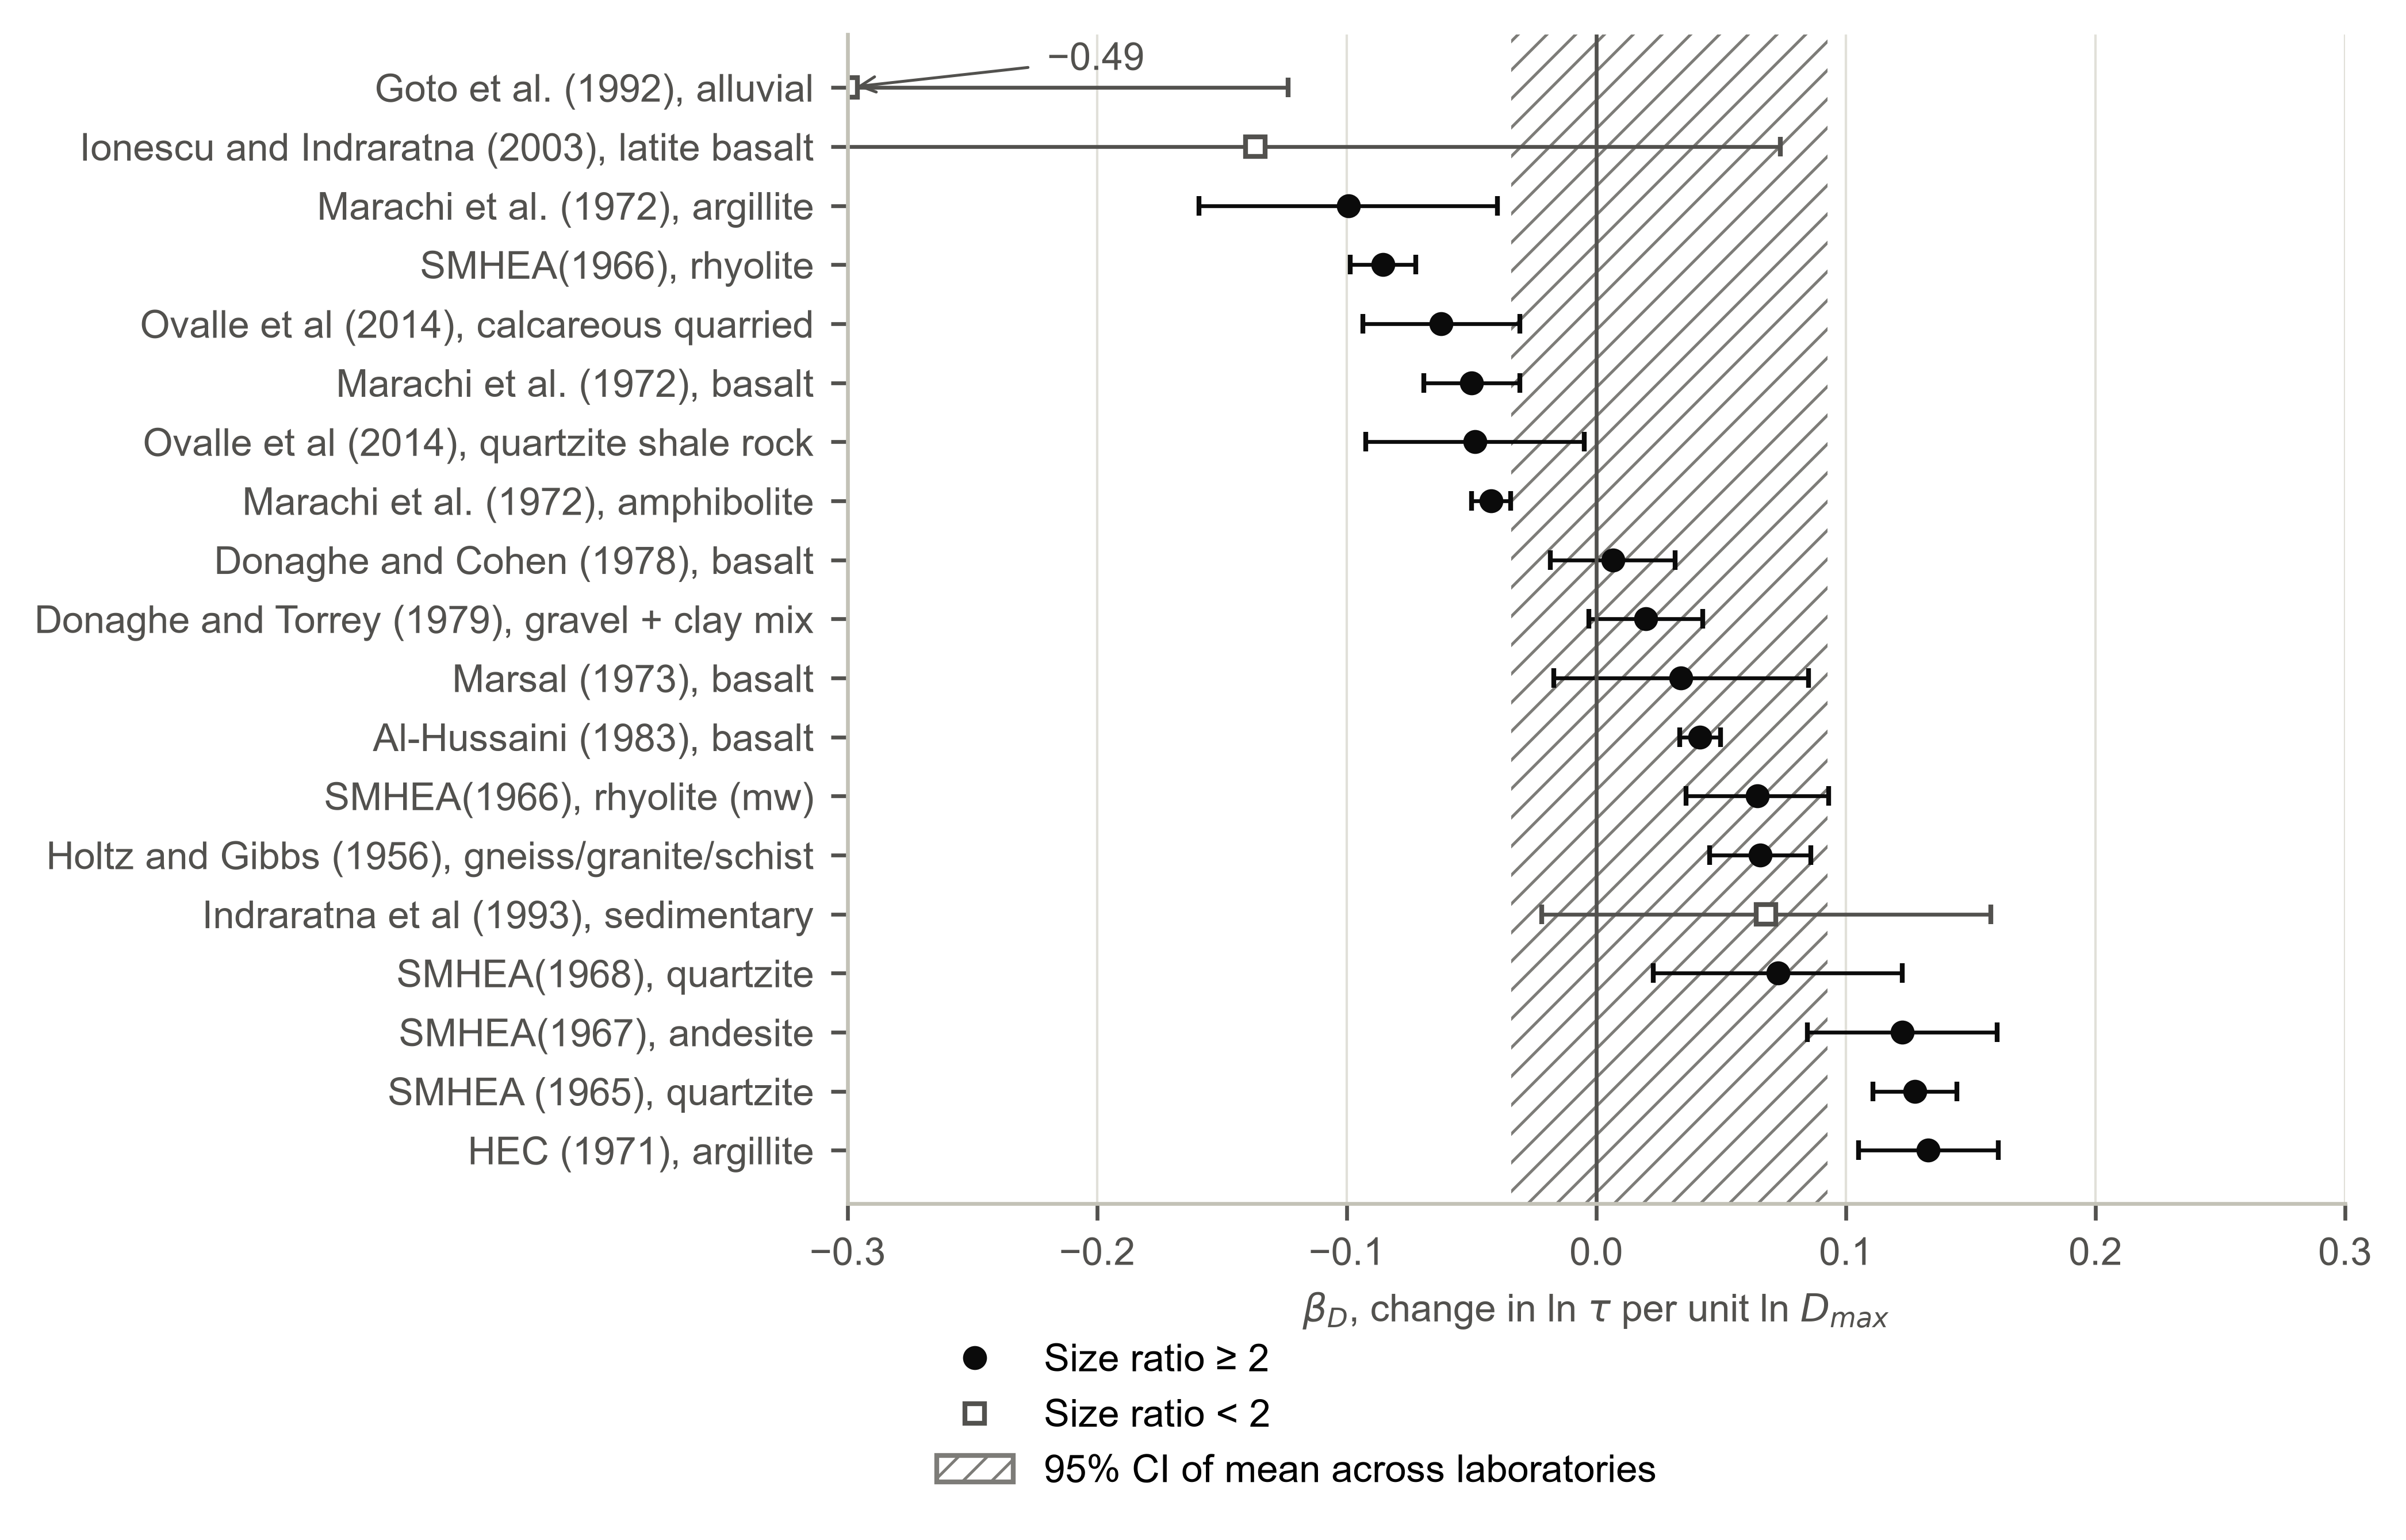
\includegraphics[width=5.6in]{FigS4_size_effect.png}
\caption{Within-material specimen-size coefficient $\beta_D$ (bars: 95\% confidence intervals; set intercepts adjusted for void ratio). Hatched band: Knapp--Hartung 95\% confidence interval of the random-effects mean across 12 publications with size ratio $\ge$ 2 (+0.041; $-$0.001 to +0.084). One value outside the axis is annotated.}
\end{figure}
\clearpage
\begin{figure}[htbp]
\centering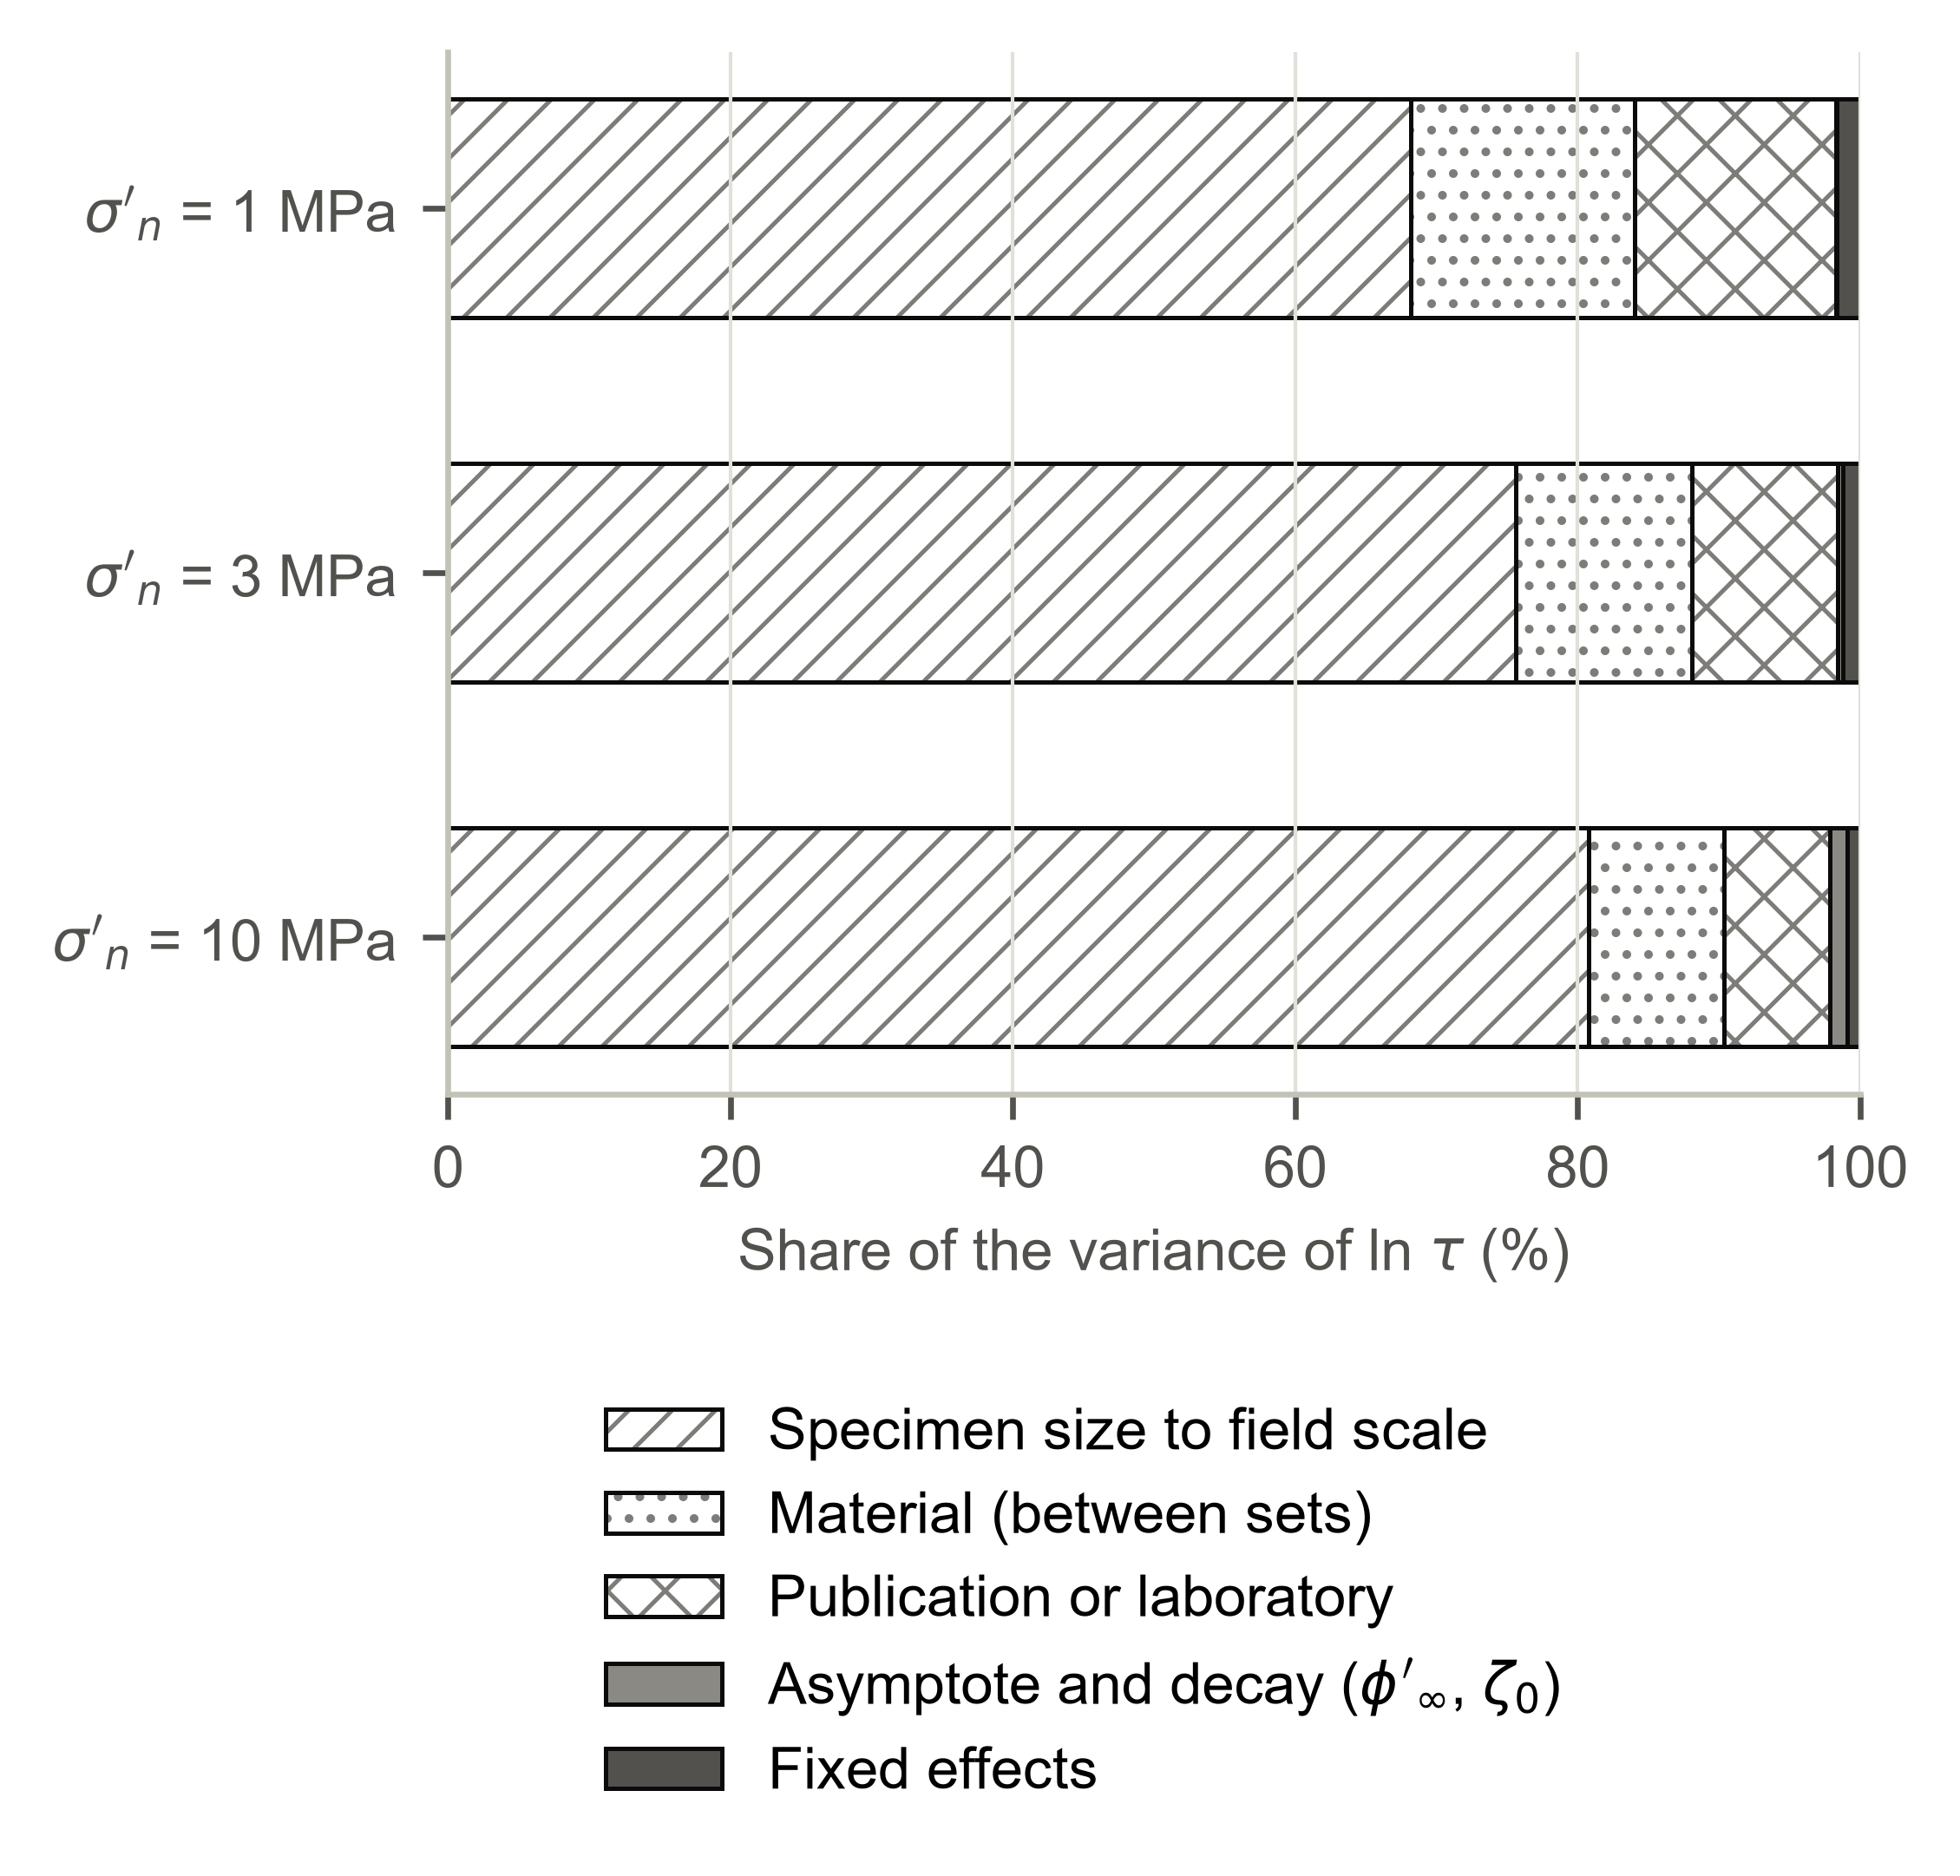
\includegraphics[width=3.5in]{FigS5_variance.png}
\caption{Shares of the variance of the mean-envelope ln $\tau$ for an untested material of low rock quality placed at e = 0.65, scaled from 0.18 m to 1 m maximum particle size.}
\end{figure}
\clearpage
\begin{table}[htbp]
\caption{Mode B: every procedure evaluated (held-out tests at $\sigma'_n$ $\ge$ 2 MPa predicted from tests at $\sigma'_n$ $\le$ 1.5 MPa of the same set)}
\centering\footnotesize
\renewcommand{\arraystretch}{1.2}
\setlength{\tabcolsep}{3.5pt}
\begin{tabular}{p{1.75in}ccccp{1.2in}p{0.55in}}
\hline\hline
Procedure & 80\% coverage & Below P10 & SD of z & CRPS & $\Delta$ vs level update (95\% CI) & Holm-adjusted p \\
\hline
Prior, no site tests & 95\% & 3\% & 0.76 & 0.0424 & +0.0115 (+0.0043 to +0.0179) & 0.48 \\
Least-squares fit of $\phi'_1$, m = 0.90 & 81\% & 17\% & 0.86 & 0.0407 & +0.0098 ($-$0.0011 to +0.0165) & 1.00 \\
Least-squares fit of $\phi'_1$, m = median within-set slope of training data & 81\% & 2\% & 1.00 & 0.0369 & +0.0061 ($-$0.0021 to +0.0207) & 0.74 \\
Joint update of both random effects & 80\% & 12\% & 1.34 & 0.0330 & +0.0022 ($-$0.0056 to +0.0200) & 1.00 \\
Level update of each set (Eq. 8) & 83\% & 9\% & 0.91 & 0.0308 & --- & --- \\
Level update after discarding flagged sets & 83\% & 12\% & 0.97 & 0.0345 & +0.0036 ($-$0.0041 to +0.0106) & 1.00 \\
Recommended procedure: discard flagged sets, joint update with shared laboratory effect & 83\% & 12\% & 0.98 & 0.0344 & +0.0036 ($-$0.0044 to +0.0104) & 1.00 \\
\hline\hline
\end{tabular}
\par\vspace{4pt}\parbox{\linewidth}{\footnotesize Note: 64 tests, 46 sets, 13 publications. The procedures were developed while examining earlier versions of the model on the same held-out sets; the comparisons are exploratory. p-values from exact sign-flip tests on publication means, Holm-adjusted within Mode B. CRPS in units of ln $\tau$.}
\end{table}
\begin{table}[htbp]
\caption{Secant friction angle $\phi'_s$ (\textdegree{}) of the waste rock of the example, median / 5th percentile of the mean envelope}
\centering\footnotesize
\renewcommand{\arraystretch}{1.2}
\setlength{\tabcolsep}{3.5pt}
\begin{tabular}{lccc}
\hline\hline
Material & Laboratory, 1 MPa & Placed, 1 MPa & Placed, 2 MPa \\
\hline
Rock type A & 40.5 / 39.1 & 35.3 / 30.3 & 33.4 / 28.6 \\
Rock type B & 43.1 / 38.6 & 38.2 / 31.5 & 35.9 / 29.8 \\
Rock type C & 41.7 / 40.3 & 37.2 / 32.0 & 35.2 / 30.2 \\
Rock type D (untested) & 40.9 / 36.6 & 36.1 / 29.5 & 34.2 / 28.0 \\
Rock type E (untested) & 40.9 / 36.5 & 33.9 / 27.4 & 32.3 / 26.3 \\
Dump average, model correlation & 41.5 / 39.7 & 36.4 / 31.1 & 34.4 / 29.4 \\
Dump average, full correlation & 41.5 / 38.7 & 36.4 / 30.6 & 34.4 / 29.0 \\
\hline\hline
\end{tabular}
\par\vspace{4pt}\parbox{\linewidth}{\footnotesize Note: Laboratory: specimen void ratio and size. Placed: void ratio 0.65 (rock type E, 0.80), maximum particle size 1 m, size effect with zero mean. The full-correlation case sorts the samples of each rock type at every stress, an upper bound on dependence. No site tests above $\sigma'_n$ $\approx$ 4.6 MPa. The critical surfaces of Table 4 of the paper mobilize $\sigma'_n$ of up to about 2 MPa.}
\end{table}
\end{document}
